\chapter{SYSTEM DESIGN }

 \section{Use case model}
\begin{figure}[H]
    \centering
    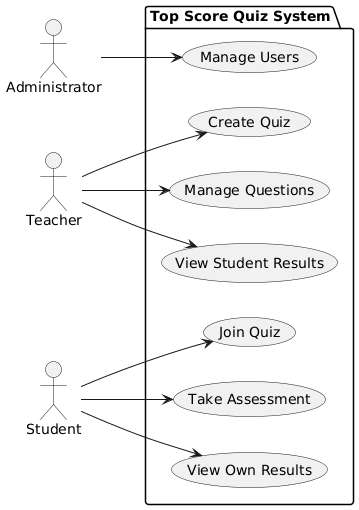
\includegraphics[width=1\textwidth,height=0.9\textwidth]{UseCase_Diagram.png}
    \caption{Use case Diagram}
    \label{fig:Use_case}
\end{figure}
This Use Case Diagram illustrates the interactions between users and the Top Score Quiz System. The Administrator manages overarching users and platform stability. The Teacher creates quizzes, adds questions, defines settings, manages quiz access codes, and reviews student results. The Student registers, joins particular quizzes using an access code, answers questions within a time constraint, submits their responses, and views instantaneous feedback.

 \section{Activity Diagram}
 \subsection{Teacher Creating Quiz}
\begin{figure}[H]
    \centering
    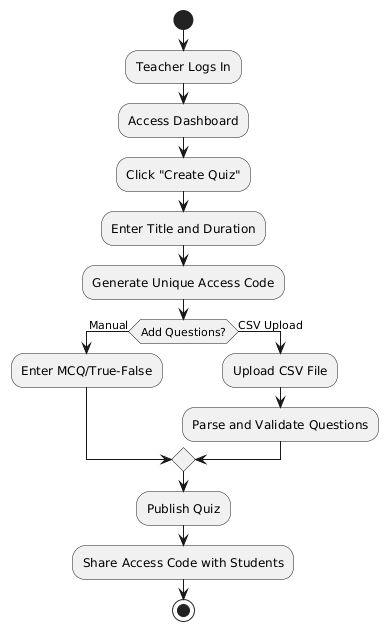
\includegraphics[width=1\textwidth,height=0.9\textwidth]{Teacher_Create_Quiz_Activity.png}
    \caption{Teacher Creating Quiz Activity diagram}
    \label{fig:Activity_1}
\end{figure}
This Activity Diagram represents the Quiz Creation process in the Top Score Quiz System. The process begins when a Teacher logs into the system and accesses the Teacher Dashboard. The Teacher selects "Create Quiz" and inputs details such as the title and duration. Upon hitting submit, a unique access code is generated automatically. Following this, the Teacher builds the quiz by manually adding questions (MCQ or True/False) or uploading a formatted CSV file. Finally, the quiz is published and the access code is shared with students.

\subsection{Student Taking Quiz}
\begin{figure}[H]
    \centering
    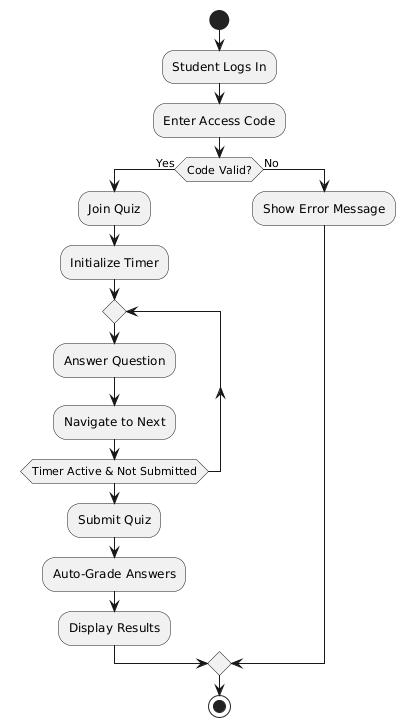
\includegraphics[width=0.5\textwidth]{Student_Take_Quiz_Activity.png}
    \caption{Student Taking Quiz Activity Diagram}
    \label{fig:Activity_2}
\end{figure}
This Activity Diagram represents the process of a Student joining and completing an assessment. The Student navigates to the Student Dashboard and inputs a provided access code. If the code is invalid, they are denied entry. If valid, the quiz environment is initialized and a countdown timer begins. The Student navigates through the questions, interacting with the system to save their responses. Once the timer expires or the Student manually submits the test, the system validates the answers against the database, immediately generates a score, and presents the final evaluation to the Student.

\section{Sequence Diagram}

\subsection{Student Quiz Submission Sequence}

\begin{figure}[H]
    \centering
    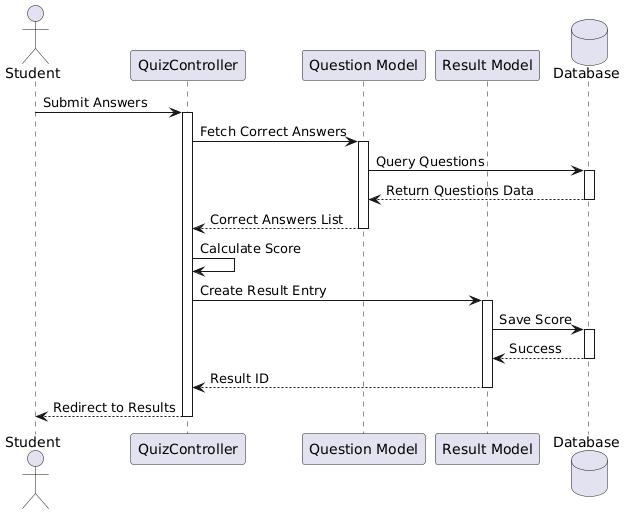
\includegraphics[width=0.9\textwidth]{Quiz_Submission_Sequence.png}
    \caption{Student Quiz Submission Sequence Diagram}
    \label{fig:Sequence_1}
\end{figure}

This sequence diagram illustrates the interaction between the Student, the QuizController, the Question Repository, and the Results Database during a quiz submission. The Student clicks "Submit" (or the timer triggers an auto-submit). The QuizController gathers the array of submitted answers and fetches the accurate 'correct\_answer' values from the Question Repository. It iterates through the student's choices, calculating the accumulated score. Finally, the total score and discrete student\_answers are logged into the Results Database, and a success response and redirect view are sent back to the Student's interface.

\section{Class Diagram}
\begin{figure}[H]
    \centering
    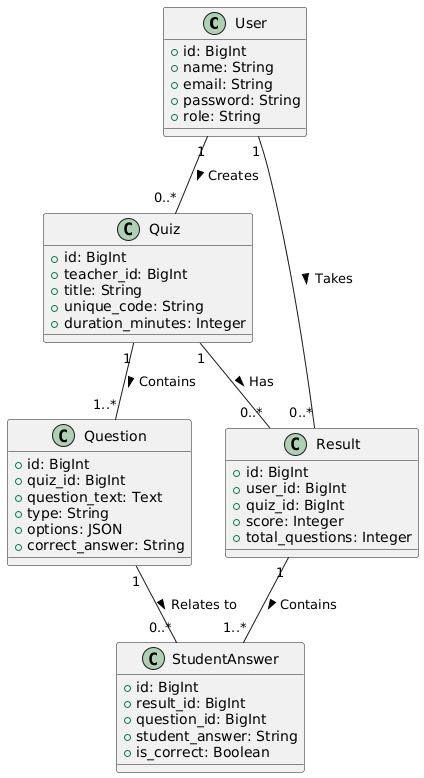
\includegraphics[width=1\textwidth]{Class_Diagram.png}
    \caption{Class Diagram}
    \label{fig:Class_Diagram}
\end{figure}
This Class Diagram represents the static structure of the Top Score Quiz System. It highlights the primary classes—such as User, Quiz, Question, and Result—along with their attributes, methods, and the relationships between them, illustrating how data is encapsulated and manipulated within the system's architecture.

\section{Entity-Relationship (ER) Diagram}
\begin{figure}[H]
    \centering
    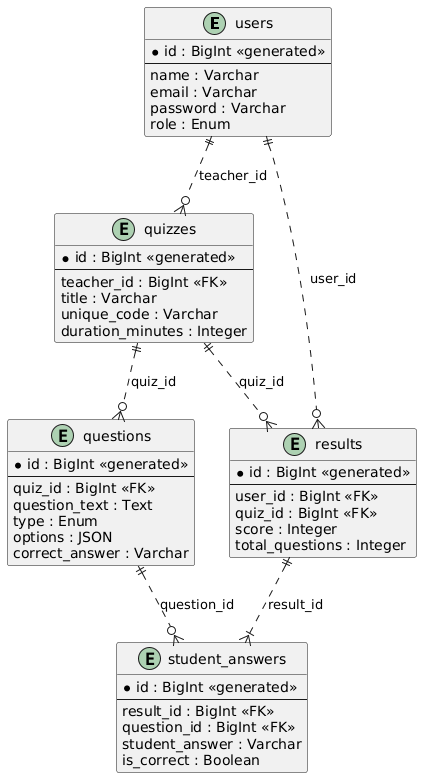
\includegraphics[width=1\textwidth,height=0.8\textwidth]{ER_Diagram.png}
    \caption{Entity-Relationship Diagram}
    \label{fig:ER_Diagram}
\end{figure}
The Entity-Relationship (ER) Diagram models the logical structure of the database. It defines the core entities—Users, Quizzes, Questions, Results, and Student Answers—and the cardinal relationships connecting them. This serves as the foundation for the relational database schema implemented in MySQL.

\section{Project Design}

System design is the process of defining the architecture, components, modules, interfaces, and data flow of a system to meet specified requirements. It ensures that the system is structured, scalable, secure, and user-friendly. Good system design focuses on usability, efficiency, performance, and data security while maintaining clear role-based responsibilities and workflow management. 

In the Top Score Quiz System, the design focuses on ensuring seamless execution of structured tests between Teachers and Students. The system integrates robust session management and data verification to maintain the academic integrity of the quizzes (e.g., verifying a user didn't modify time constraints). The system balances complex underlying evaluations with a streamlined dashboard experience for ease of use.

\subsection{UI Design}

The User Interface (UI) design of Top Score is structured to be distraction-free, modern, and purely functional. Each user type—Admin, Teacher, and Student—has a distinct dashboard displaying relevant tools.

\begin{figure}[H]
    \centering
    \includegraphics[width=1\textwidth]{image_0.png}
    \caption{Landing / Login Interface}
    \label{fig:Screenshot_1}
\end{figure}

The UI includes:
\begin{itemize}
    \item A streamlined Student interface emphasizing active quizzes, a prominent join-code input, and clear visual timers during assessments.
    \item A comprehensive Teacher dashboard displaying a list of their owned quizzes, tools to manage questions, and detailed tabular formats for student result evaluations.
    \item Clean authentication forms and straightforward navigational menus adhering to contemporary frontend standards.
\end{itemize}

\begin{figure}[H]
    \centering
    \includegraphics[width=1\textwidth]{image_1.png}
    \caption{Teacher Dashboard}
    \label{fig:Screenshot_2}
\end{figure}

\begin{figure}[H]
    \centering
    \includegraphics[width=1\textwidth]{image_4.png}
    \caption{Student Dashboard}
    \label{fig:Screenshot_5}
\end{figure}

\subsection{User Interaction Design}

The system is engineered for prompt feedback. Interactions like joining a quiz validate access codes synchronously and throw immediate alerts if incorrect. When a student takes a quiz, the system actively updates them on their remaining time and allows them to navigate questions flexibly before the final submission.

\begin{figure}[H]
    \centering
    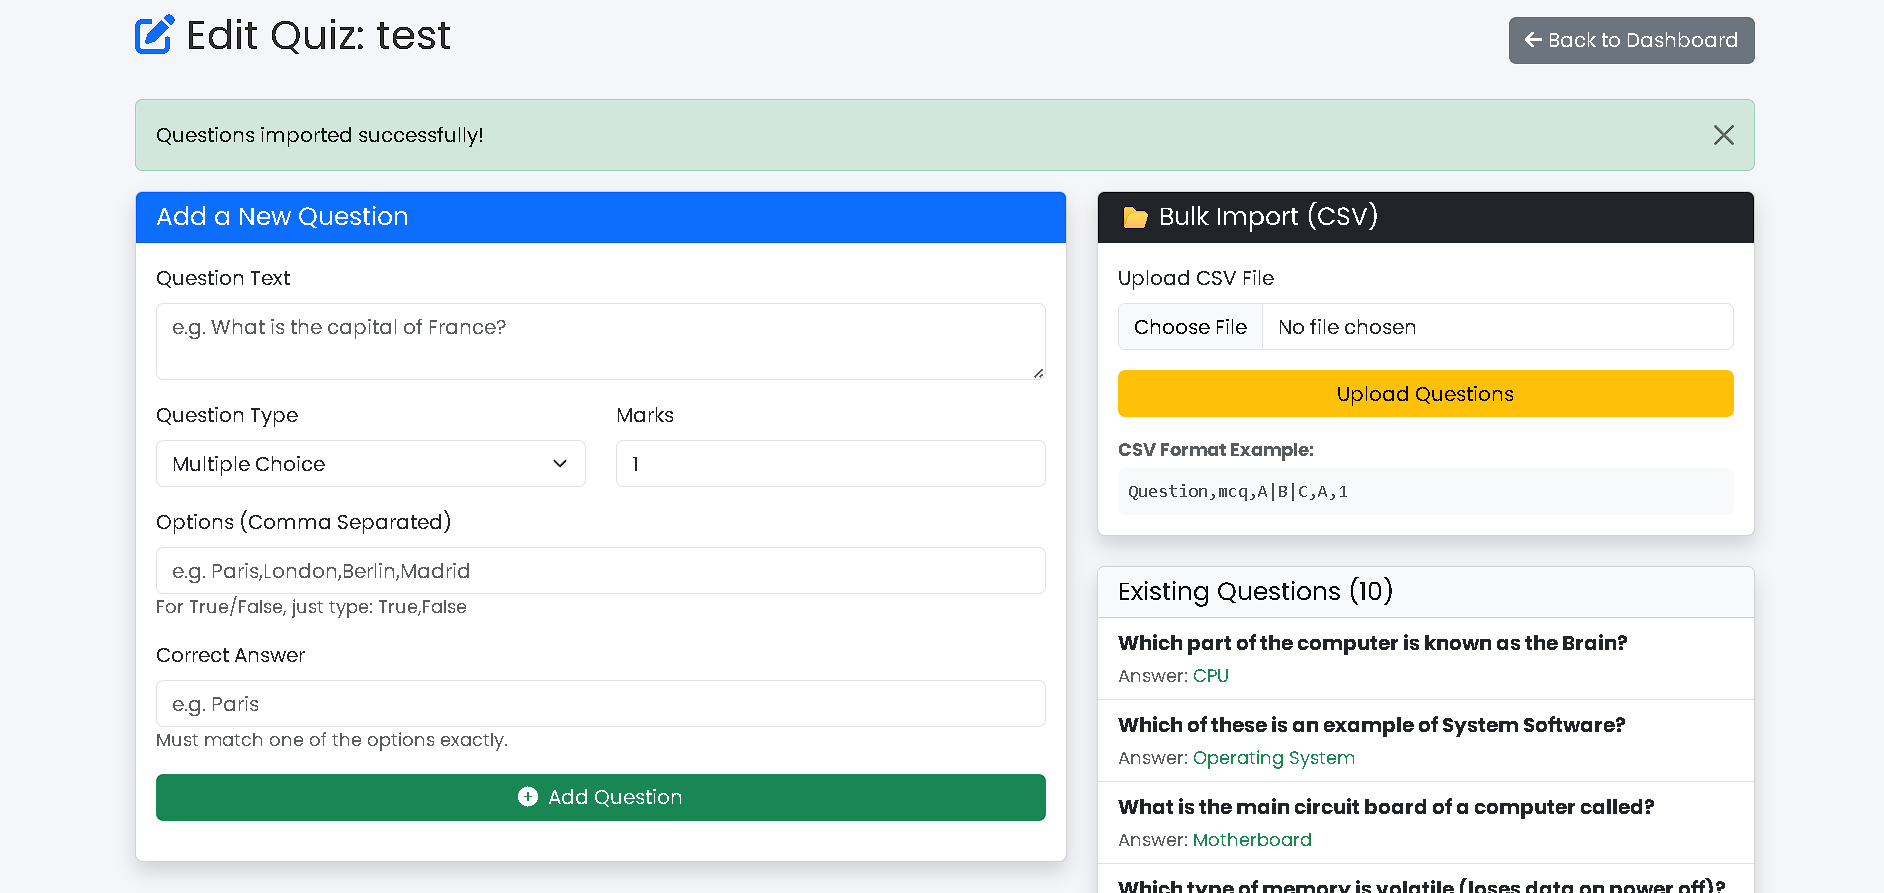
\includegraphics[width=1\textwidth]{quiz creation.png}
    \caption{Teacher Quiz Creation Page}
    \label{fig:Screenshot_3}
\end{figure}

Role-based interaction ensures:
\begin{itemize}
    \item Students are sandboxed within their active attempts and previous results summaries.
    \item Teachers control the pacing and distribution of their instructional material.
    \item Accidental double-submissions are mitigated through prompt UI state changes and controller-level restrictions upon pressing "Submit."
\end{itemize}

\subsection{Grading and Evaluation Design}

The system uses a synchronous grading algorithm executed entirely on the server side to prevent tampering. Every question carries a designated weight/mark (defaulting to 1). Upon submission, the student's payload is evaluated rigorously against the stored correct answers. The resulting metadata, including total points, potential grades (e.g., Pass/Fail threshold), and individual erroneous answers, are stored persistently for identical post-test reviews for both Student and Teacher.

\begin{figure}[H]
    \centering
    \includegraphics[width=1\textwidth]{image_3.png}
    \caption{Teacher - Class Performance Metrics}
    \label{fig:Screenshot_4}
\end{figure}

\subsection{Project Pipeline}
The project pipeline outlines the systematic flow from initial HTTP request to database transaction and back to the client interface. The standard Laravel architecture handles this through the following steps:
\begin{enumerate}
    \item \textbf{Routing:} Incoming HTTP requests are intercepted by \texttt{web.php} and mapped to appropriate Controller methods.
    \item \textbf{Middleware:} Authentication and role-based checks (e.g., verifying Teacher vs. Student roles) are enforced before execution.
    \item \textbf{Controller Logic:} The designated Controller processes the request, validates input data, and triggers necessary business logic.
    \item \textbf{Model \& Database Interaction:} Eloquent ORM Models interact securely with the MySQL database to retrieve or store information dynamically.
    \item \textbf{View Rendering:} The Controller passes formatted data to Blade templates to construct the frontend HTML presentation logically.
\end{enumerate}

\subsection{Database Design}

The database design follows a strict relational structure using MySQL. The system consists of standard framework tables (\texttt{cache}, \texttt{cache\_locks}, \texttt{failed\_jobs}, \texttt{job\_batches}, \texttt{jobs}, \texttt{migrations}, \texttt{password\_reset\_tokens}, \texttt{sessions}) and primary system entities. The core tables are elaborated in the data dictionary below:

\subsubsection{Data Dictionary}

\begin{table}[H]
    \centering
    \begin{tabular}{|l|l|l|}
        \hline
        \textbf{Column Name} & \textbf{Data Type} & \textbf{Description} \\
        \hline
        id & BigInt, Auto Increment & Primary Key \\
        name & Varchar(255) & User's full name \\
        email & Varchar(255) & Unique email address \\
        password & Varchar(255) & Hashed password \\
        role & Enum('admin', 'teacher', 'student') & Role for access control \\
        created\_at & Timestamp & Record creation time \\
        updated\_at & Timestamp & Record modification time \\
        \hline
    \end{tabular}
    \caption{Users Table}
    \label{tab:users}
\end{table}

\begin{table}[H]
    \centering
    \begin{tabular}{|l|l|l|}
        \hline
        \textbf{Column Name} & \textbf{Data Type} & \textbf{Description} \\
        \hline
        id & BigInt, Auto Increment & Primary Key \\
        teacher\_id & BigInt & Foreign Key (Users) \\
        title & Varchar(255) & Title of the quiz \\
        unique\_code & Varchar(10) & Unique code to join quiz \\
        duration\_minutes & Integer & Total time for the quiz \\
        created\_at & Timestamp & Record creation time \\
        updated\_at & Timestamp & Record modification time \\
        \hline
    \end{tabular}
    \caption{Quizzes Table}
    \label{tab:quizzes}
\end{table}

\begin{table}[H]
    \centering
    \begin{tabular}{|l|l|l|}
        \hline
        \textbf{Column Name} & \textbf{Data Type} & \textbf{Description} \\
        \hline
        id & BigInt, Auto Increment & Primary Key \\
        quiz\_id & BigInt & Foreign Key (Quizzes) \\
        question\_text & Text & The actual question \\
        type & Enum('mcq', 'true\_false') & Type of question \\
        options & JSON & JSON array of options \\
        correct\_answer& Varchar(255) & Correct option / answer \\
        created\_at & Timestamp & Record creation time \\
        updated\_at & Timestamp & Record modification time \\
        \hline
    \end{tabular}
    \caption{Questions Table}
    \label{tab:questions}
\end{table}

\begin{table}[H]
    \centering
    \begin{tabular}{|l|l|l|}
        \hline
        \textbf{Column Name} & \textbf{Data Type} & \textbf{Description} \\
        \hline
        id & BigInt, Auto Increment & Primary Key \\
        user\_id & BigInt & Foreign Key (Users) \\
        quiz\_id & BigInt & Foreign Key (Quizzes) \\
        score & Integer & Total score obtained \\
        total\_questions & Integer & Total questions in quiz \\
        created\_at & Timestamp & Record creation time \\
        updated\_at & Timestamp & Record modification time \\
        \hline
    \end{tabular}
    \caption{Results Table}
    \label{tab:results}
\end{table}

\begin{table}[H]
    \centering
    \begin{tabular}{|l|l|l|}
        \hline
        \textbf{Column Name} & \textbf{Data Type} & \textbf{Description} \\
        \hline
        id & BigInt, Auto Increment & Primary Key \\
        result\_id & BigInt & Foreign Key (Results) \\
        question\_id & BigInt & Foreign Key (Questions) \\
        student\_answer& Varchar(255) & The option selected \\
        is\_correct & Boolean & If answer was correct \\
        created\_at & Timestamp & Record creation time \\
        updated\_at & Timestamp & Record modification time \\
        \hline
    \end{tabular}
    \caption{Student Answers Table}
    \label{tab:student_answers}
\end{table}

Each entity relies heavily on cascading foreign-key relationships to ensure data consistency (e.g., removing a Quiz automatically flushes associated Questions and local Results). 

\subsection{Workflow Design}

The structural workflow guarantees an intuitive instructional process:

\begin{itemize}
    \item A Teacher logs in, creates a quiz, and receives the auto-generated join code.
    \item The Teacher inserts questions into the Quiz manually or via bulk CSV mechanisms.
    \item The Teacher distributes the access code independently to the target class.
    \item A Student inputs the unique code on their dashboard to enroll.
    \item The Student undertakes the test under a strict timer constraint.
    \item Upon conclusion, the system executes an automated grading protocol and saves the result.
    \item The Student views an immediate personal review, while the Teacher views an aggregated classroom report.
\end{itemize}


